\subsection{Creazione di una prenotazione}

\begin{figure}[H]
  \centering
    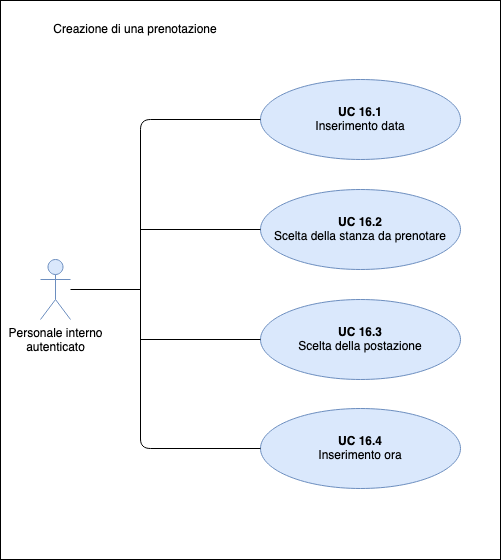
\includegraphics[width=\textwidth]{src/CasiDUso/immagini/UC-creazionePrenotazione.png}
  \caption{Creazione di una prenotazione}
\end{figure}

Il presente diagramma vuole riassumere la possibilità di gestione delle prenotazioni da parte di un utente autenticato nell’applicazione.

\begin{itemize}
\item \textbf{Attori primari:} personale interno autenticato;
\item \textbf{Descrizione:} il personale interno autenticato vuole gestire una prenotazione a cui ha accesso a livello di permessi, con possibilità di creazione, modifica, eliminazione e visualizzazione;
\item \textbf{Precondizione:} il personale interno è autenticato nell’applicazione e ha i permessi per eseguire le azioni di cui sopra;
\item \textbf{Postcondizione:} il personale interno autenticato ha creato, modificato, eliminato o visualizzato una prenotazione;
\item \textbf{Scenario principale:} 
	\begin{itemize}
		\item il personale interno naviga nell’apposita sezione di modifica della prenotazione;
		\item il personale interno crea, visualizza, modifica o rimuove una sua prenotazione;
		\item la prenotazione passa in stato di “pending” e, dopo una serie di controlli, viene confermata o eliminata.
	\end{itemize}
\end{itemize}

\subsection{UC-16 Creazione di una prenotazione}

\begin{itemize}
\item \textbf{Attori primari:} personale interno autenticato;
\item \textbf{Descrizione:} l'attore vuole prenotare una postazione per una certa data od orario scelti;
\item \textbf{Precondizione:} l'attore naviga nell’apposita sezione di creazione di una prenotazione, visualizzando a video la lista delle postazioni con relativi orari prenotabili;
\item \textbf{Postcondizione:} l'attore crea correttamente una prenotazione per la data ed ora scelta;
\item \textbf{Scenario principale:} 
	\begin{itemize}
		\item l'attore seleziona la data in cui desidera prenotare una postazione[UC-16.1];
		\item l'attore seleziona la stanza in cui vuole prenotare una postazione dalla lista delle stanze abilitate[UC-16.2];
		\item l'attore visualizza la lista di postazioni prenotabili nella stanza selezionata per la data precedentemente selezionata;
		\item l'attore seleziona la postazione che desidera prenotare[UC-16.3];
		\item l'attore seleziona l'orario della prenotazione tra la lista degli orari in cui la prenotazione è libera ed igienizzata[UC-16.4];
		\item il sistema elabora correttamente la richiesta, mandando in stato di “pending” la prenotazione;
	\end{itemize}
\end{itemize}

\subsubsection{UC-16.1 Inserimento data}

\begin{itemize}
\item \textbf{Attori primari:} personale interno autenticato;
\item \textbf{Descrizione:} l'attore vuole inserire la data in cui prenotare una postazione;
\item \textbf{Precondizione:} l'attore seleziona una data valida dal calendario;
\item \textbf{Postcondizione:} l'attore seleziona correttamente una data dal calendario;
\item \textbf{Scenario principale:} il sistema elabora correttamente la richiesta;
\end{itemize}

\subsubsection{UC-16.2 Scelta della stanza da prenotare}

\begin{itemize}
\item \textbf{Attori primari:} personale interno autenticato;
\item \textbf{Descrizione:} l'attore vuole selezionare la stanza in cui prenotare una postazione;
\item \textbf{Precondizione:} l'attore seleziona una stanza valida dalla lista delle stanze disponibili ed attive;
\item \textbf{Postcondizione:} l'attore seleziona correttamente una stanza;
\item \textbf{Scenario principale:} il sistema elabora correttamente la richiesta;
\end{itemize}

\subsubsection{UC-16.3 Scelta della postazione da prenotare}

\begin{itemize}
\item \textbf{Attori primari:} personale interno autenticato;
\item \textbf{Descrizione:} l'attore vuole selezionare una postazione valida dalla lista delle postazioni disponibili, attive ed igienizzate;
\item \textbf{Precondizione:} l'attore seleziona una postazione valida dalla lista;
\item \textbf{Postcondizione:} l'attore seleziona correttamente una postazione valida;
\item \textbf{Scenario principale:} il sistema elabora correttamente la richiesta;
\end{itemize}

\subsubsection{UC-16.4 Inserimento ora}

\begin{itemize}
\item \textbf{Attori primari:} personale interno autenticato;
\item \textbf{Descrizione:} l'attore vuole inserire l'orario in cui prenotare una postazione;
\item \textbf{Precondizione:} l'attore seleziona un orario valido dalla lista degli orari disponibili per la postazione precedentemente selezionata;
\item \textbf{Postcondizione:} l'attore seleziona correttamente un orario disponibile;
\item \textbf{Scenario principale:} il sistema elabora correttamente la richiesta.
\end{itemize}

%\subsubsection{UC-1.1 - Visualizzazione errore di prenotazione: prenotazione per determinata fascia oraria già esistente}
%\begin{itemize}
%\item \textbf{Attori primari:} personale interno autenticato;
%\item \textbf{Precondizione:} il personale interno sta cercando di prenotare una postazione in una data ed orario in cui la postazione risulta già prenotata da un altro utente;
%\item \textbf{Postcondizione:} la prenotazione non viene approvata ed il personale interno autenticato riceve un messaggio di errore auto-esplicativo;
%\item \textbf{Scenario principale:} il personale interno autenticato visualizza un messaggio di errore in cui viene informato che la postazione risulta già occupata per la data e ora da lui scelti.
%\end{itemize}

%\subsubsection{UC-1.2 - Visualizzazione errore di prenotazione: postazione disabilitata da un amministratore}
%\begin{itemize}
%\item \textbf{Attori primari:} personale interno autenticato;
%\item \textbf{Precondizione:} il personale interno autenticato sta cercando di prenotare una postazione che risulta essere stata disabilitata da un amministratore;
%\item \textbf{Postcondizione:} la prenotazione non viene approvata e il personale interno autenticato riceve un messaggio di errore auto-esplicativo;
%\item \textbf{Scenario principale:} il personale interno autenticato visualizza un messaggio di errore in cui viene informato che la postazione risulta disabilitata e quindi non prenotabile.
%\end{itemize}


\subsection{UC-17 Modifica di una prenotazione}

\begin{itemize}
\item \textbf{Attori primari:} personale interno autenticato;
\item \textbf{Descrizione:} l'attore vuole modificare una postazione per una certa data ed orario;
\item \textbf{Precondizione:} l'attore naviga nell’apposita sezione di modifica di una prenotazione;
\item \textbf{Postcondizione:} l'attore modifica correttamente una prenotazione per la nuova data/ora scelta;
\item \textbf{Scenario principale:} 
	\begin{itemize}
		\item l'attore seleziona la nuova data in cui desidera prenotare una postazione[UC-1.1];
		\item l'attore seleziona la nuova stanza in cui vuole prenotare una postazione dalla lista delle stanze abilitate[UC-1.2];
		\item l'attore visualizza la lista di postazioni prenotabili nella stanza selezionata per la nuova data precedentemente selezionata;
		\item l'attore seleziona la nuova postazione che desidera prenotare[UC-1.3];
		\item l'attore seleziona il nuovo orario della prenotazione tra la lista degli orari in cui la prenotazione è libera ed igienizzata[UC-1.4];
		\item il sistema elabora correttamente la richiesta, mandando in stato di “pending” la prenotazione;
	\end{itemize}
\end{itemize}

\subsection{UC-18 Cancellazione di una prenotazione}

\begin{itemize}
\item \textbf{Attori primari:} personale interno autenticato;
\item \textbf{Descrizione:} l'attore vuole cancellare una prenotazione per una certa data ed orario effettuata in precedenza;
\item \textbf{Precondizione:} l'attore naviga nell’apposita sezione di cancellazione di una prenotazione;
\item \textbf{Postcondizione:} l'attore cancella correttamente la prenotazione per la data/ora scelta;
\item \textbf{Scenario principale:} 
	\begin{itemize}
		\item il sistema elabora correttamente la richiesta;
		\item il sistema restituisce un errore per i seguenti motivi:
		\begin{itemize}
			\item non è possibile cancellare una prenotazione per un orario passato[UC-3.1].
		\end{itemize}
	\end{itemize}
\end{itemize}

\subsubsection{UC-18.1 Visualizzazione errore di cancellazione: tentativo di cancellazione di una prenotazione per un orario passato}
\begin{itemize}
\item \textbf{Attori primari:} personale interno autenticato;
\item \textbf{Precondizione:} il personale interno autenticato sta cercando di cancellare una prenotazione già usufruita in un orario passato;
\item \textbf{Postcondizione:} la cancellazione non viene approvata e il personale interno auteneticato riceve un messaggio di errore auto-esplicativo;
\item \textbf{Scenario principale:} il personale interno autenticato visualizza un messaggio di errore in cui viene informato che non è possibile cancellare una prenotazione per un orario passato.
\end{itemize}

\subsection{UC-19 Visualizzazione di una prenotazione}

\begin{itemize}
\item \textbf{Attori primari:} personale interno autenticato;
\item \textbf{Descrizione:} l'attore vuole visualizzare le sue prenotazioni attive nel sistema;
\item \textbf{Precondizione:} l'attore naviga nell’apposita sezione di visualizzazione delle sue prenotazioni;
\item \textbf{Postcondizione:} l'attore visualizza correttamente le sue prenotazioni attive;
\item \textbf{Scenario principale:} 
	\begin{itemize}
		\item il sistema elabora correttamente la richiesta e, nel caso in cui non ci sia una prenotazione attiva, visualizzerà un form vuoto in cui si informerò l'utente che non si ha alcuna prenotazione attiva.
	\end{itemize}
\end{itemize}


%\subsubsection{UC-4.1 - Visualizzazione errore di prenotazione attiva: l'utente non ha alcuna prenotazione attiva}
%\begin{itemize}
%\item \textbf{Attori primari:} personale interno autenticato;
%\item \textbf{Precondizione:} il personale interno auteneticato sta cercando di visualizzare la lista delle sue prenotazioni, non avendone però alcuna attiva;
%\item \textbf{Postcondizione:} la visualizzazione non viene eseguita e il personale interno autenticato riceve un messaggio di errore auto-esplicativo;
%\item \textbf{Scenario principale:} il personale interno autenticato visualizza un messaggio di errore in cui viene informato che non ha alcuna prenotazione attiva.
%\end{itemize}